\section{Background and Preliminaries} \label{sec:background}
%%This section reviews several key concepts for our proposed computational machine self-confidence framework. To make the concepts discussed throughout the paper concrete and provide an accessible proof-of-concept testbed in later sections, we also describe a motivating APS application example inspired by ongoing research in unmanned robotic systems.  
%%\nisar{for me todo: refactor this section: start with overview of what will be covered, then talk about MDPs more formally and give details for reward, etc.; map Donut Delivery application to other robotic autonomous system applications -- note that Donut Delivery will be revisited in Experiments with users later as a basic test (can maybe include user's go/no-go call in Figure 1 somehow?)... VERY IMPORTANT: NEED TO ADD RELATED/PRIOR WORK SECTION!! need to discuss limitations and motivate why \famsec{} is needed !! Then section 3 should be \famsec{}, with first big subsection on \xO{} and second big subsection on \xQ{} (with numerical examples)...section 4 experiments, with details (e.g. of how sim generated/typical reward dists and road nets) and extended results...section 5 discussion, section 6 conclusions...}

\subsection{Related Work}
%%\nisar{formal methods? good for checking specifications, but specifications are hard to formulate and understand for joe sixpack...}
%%Moving to Sec. II:
As distinct from research on autonomous introspection for self-improvement \cite{Paul2011-vr, Triebel2013-ow,Triebel2016-kj}, 
we are not motivated here by whether/how a robot can adapt its functional capabilities to \emph{improve} its performance on a particular task -- but rather by the more basic question of whether a robot has a `reasonable' or contextually useful understanding of how its current functional capabilities would lead it to \emph{actually} perform on that task. As an analogy: consider how, say, a correctly tuned Kalman filter can be trusted to `know' its true state error statistics through the computed state error covariance matrix (i.e. such that the assumed approximate filtering distribution model can be statistically validated by truth model simulations and correctly fits actual sensor data) \cite{Bar-Shalom2001-tg}. We argue here that a robot with a correct sense of `self-trust' could also be similarly trusted to know its own performance limitations on a given task --- provided that the self-trust measure actually reflects how well the robot's underlying functionality (with all the attendant models, data, assumptions, algorithms, and other programmed/pre-ordained approximations of reality) fits the task. As such, we primarily seek to explore and establish meaningful self-trust measures. 

Our work can also be contrasted to recent work on explainable/interpretable learning and AI \cite{Huang2018-ab,Lipton2016-ug,Ribeiro2016-uc,Guidotti2018-pi}, where the aim primarily is to enable the robot to provide some tailored form of post hoc justification, summary, or notification of critical actions/states encountered, after/while the robot performs a task already delegated to it (often alongside a co-equal human partner). In our work, we want to understand whether and how the robot could assess \emph{on its own} if the task that could be delegated to it by a human supervisor (i.e. not a co-equal) falls within its competency boundaries, and thus whether the task to be delegated is even appropriate for or realistically achievable by that robot in the first place. %(thus potentially altogether avoiding the need for in situ/post hoc explanations of critical actions/states). 
%or research on explainable/interpretable learning and AI \cite{bunchofstuff}

These considerations naturally lead to algorithmic meta-analysis of autonomy, i.e. analysis and assessment of the processes used to define and implement autonomous functional abilities. This builds on the concept of `machine self-confidence' put forth by \cite{Hutchins2015-if}, which proposed using human expert evaluations of specific autonomous system capabilities to manually encode where and when these may break down in particular tasking situations. However, as argued above: to be useful and scalable for real applications, autonomous robots should be able to form such assessments on their own. While several definitions and algorithmic approaches have been proposed recently for specific applications \cite{ Kuter2015-qh,Sweet2016-tz,  Zagorecki2015-qy}, these do not support general functional capabilities for decision-making under uncertainty. 
%
%we restrict attention to the following general definition of self-confidence: \textit{an agent's perceived ability to achieve assigned goals (within a defined region of autonomous behavior) after accounting for (1) uncertainties in its knowledge of the world, (2) uncertainties of its own state, and (3) uncertainties about its reasoning process and execution abilities.} %\nisar{can move prev sent to \famsec{} section?} 


\begin{figure}[t]%[htbp]
    	\centering
     	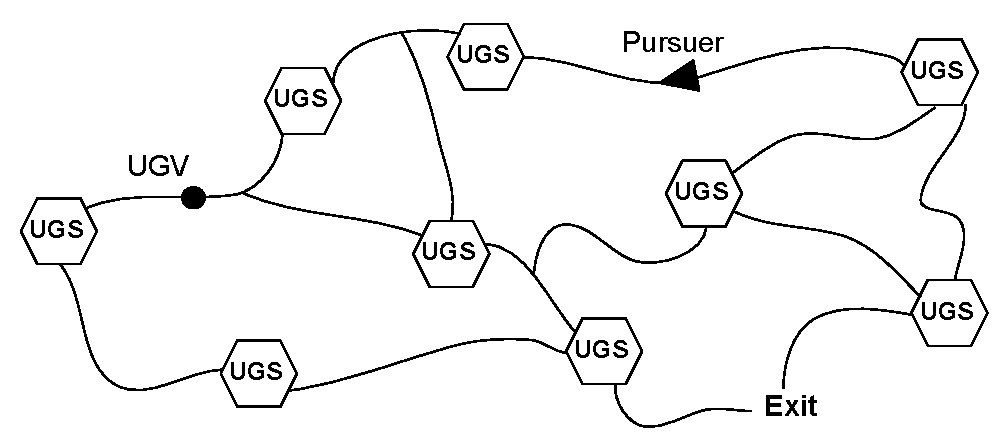
\includegraphics[width=0.4\textwidth]{Figures/RoadNet}
    	\caption{Road network for Donut Delivery problem.} 
        \label{fig:RoadNet}
        \vspace{-0.2cm}
\end{figure}    


\subsection{Autonomous Planning and Decision-making with MDPs} \label{sec:mdp}
%%The diversity of factors that influence APS self-confidence requires a rich modeling approach for algorithmic assessment. 
Our examination of algorithmic self-confidence assessments will primarily focus on autonomous planning and decision-making capabilities modeled as Markov decision processes (MDPs). %%MDPs are composed of finite states and actions that partially resolve the nondeterminism in state transitions by deciding from what probability distribution the next state will be sampled. %%The co-existence of nondeterministic and stochastic choices in MDPs are expressive enough to account for a range of uncertainties including adversarial environmental factors and inaccuracies in execution. %%, and limitations in prior knowledge (e.g. imperfect knowledge of $p(\cdot)$).  
MDPs have well-established connections to other widely used approaches for autonomous decision-making and learning under uncertainty, such as partially observable MDPs (POMDPs) for decision-making in limited observability environments and reinforcement learning for decision-making with incomplete model information \cite{Kochenderfer2015-uu}. As such, they provide an ideal starting point for an initial analysis of self-confidence that can be generalized in future work. 

We consider generic MDP formulations of a delegated task \task{} by a human supervisor (user) to an autonomous robot. In an MDP framing of \task{}, the autonomous agent must find an optimal policy $\pi = u(x)$ for an MDP with dynamical state $x$ and actions $u$, such that the objective function
$U = \mathbb{E} \left[\sum_{k=0}^{\infty} \gamma^k r(x_k,u_k) \right]$ is maximized for all times $k=0,...,\infty$ --  
where $R(x_k,u_k)$ rewards (penalizes) the robot for being in (un)desirable states and taking (un)desirable actions, $\mathbb{E}[\cdot]$ is the expected value over all possible future states, and $\gamma \in (0,1]$ is a fixed future discount factor. 
Given any $u_k$, the state $x_k$ updates via a Markov probabilistic transition model $x_{k+1} \sim p(x_{k+1}|x_{k},u_{k})$,  
i.e. $x_{i}$ is fully observed at time $i$ (no sensor noise), while transitions $i\rightarrow k+1$ have random perturbations.
In a fully posed MDP, $\pi$ is the optimal state-action policy, which can be recovered from Bellman's equation via dynamic programming. 
However, in many practical cases, policy approximations $\tilde{\pi}$ are required to cope with complex or uncertain dynamics (e.g. using reinforcement learning or policy approximations for very large state spaces) \cite{Kochenderfer2015-uu}. 

\subsection{Donut Delivery Application} \label{sec:donut_delivery}
We use the `Donut Delivery' problem (based on the `VIP escort' scenario~\cite{Humphrey2012-lr}) as a concrete grounding example. As shown in Fig.~\ref{fig:RoadNet}, an autonomous donut delivery truck (ADT) navigates a road network in order to reach a delivery destination while avoiding a motorcycle gang (MG) that will steal the donuts if they cross paths with the delivery truck. The motorcycle gang's location is unknown but can be estimated using intermittent updates from unmanned ground sensors (UGS). The delivery truck's decision space involves selecting a sequence of discrete actions (i.e. go straight, turn left, turn right, go back, stay in place). The ADT motion, UGS readings, and MG behavior are stochastic, and the problems of decision making and sensing are strongly coupled: some trajectories through the network might allow the ADT to localize the MG before heading to the delivery destination but incur a high time penalty); other trajectories may afford rapid delivery with high MG location uncertainty but increase the risk of getting caught by the MG, which can take multiple paths. A human supervisor monitors the ADT during operation. The supervisor does not have detailed knowledge or control of the ADT---but can  (based on whatever limited information is available) decide to proceed with or abort the delivery before it starts. 
%, as well as potentially modify its decision making stance (`aggressively pursue exit' vs. `be very conservative and cautious') in order to better cope with the MG (which is sporadically observed and follows an unknown course). \nisar{modify last sentence -- just state go/no go?}

The physical states describing the combined location of the ADT (whose states are always perfectly observable) and MG can be discretized in time and space to produce a Markov process model defined by some initial joint state probability distribution and joint state transition matrix, which depends on the navigation actions taken by the ADT (e.g. move to the nearest neighboring intersection).
%The probability of obtaining `detection' and `no detection' data from each UGS given the true state of the MG can be modeled and used to update probabilistic beliefs about the MG's state. 
%Finally, 
A reward function $R(x_k,u_k) = R_k$ can be specified for each time step $k$ to encode user preferences over the combined state of the ADT and MG, e.g. $R_k = -200$ for each time step the ADT is not co-located with the MG but not yet at the goal, $R_k= -2000$ if the ADT and MG are co-located, and $R_k=+2000$ if the ADT reaches the goal without getting caught. 
%Given these elements, the ADT's navigational planning and decision-making problem may be generally formulated as a POMDP. 
%If the MG's state is fully observable at each step $k$ (e.g. due to very reliable and accurate UGS that cover all areas of the road network), the problem reduces to an MDP. 
Assuming the MG's state is observable at each step $k$ (due to very reliable and accurate UGS that cover all areas of the road network), the ADT's planning problem can be treated as an MDP. 


% %%%%%%%%%%%%%%%%%%%%%%
% %%%OLD:
% %%\nisar{VERY IMPORTANT: add subsection to expand on related work: esp. Dragan's critical states and Srinivasa's trust POMDPs, other versions of self-confidence -- need to discuss limitations and motivate why \famsec{} is needed !! Might also be good to justify why a meta-analysis framework is appropriate...}
% The problem of identifying and designing algorithmic assurances for trust calibration in human-autonomous robot interaction is deeply connected to the growing literature on explainable/interpretable AI and machine learning \nisar{(refs)}, as well as established and ongoing human factors research on trust in automated systems \nisar{(refs)}. 
% Ref. \cite{Israelsen2018-qz} provides a comprehensive survey on these connections. 
% To motivate the concept of machine self-confidence, we highlight a few recent developments from the algorithmic assurance and autonomous robotics literature that are most closely related to the present work. 

% Building on the trust cycle and analysis framework of McKnight, et al. \nisar{[cite]}, ref. \cite{Israelsen2018-qz} notes that all practical algorithmic assurances attempt to calibrate one or more `trustworthiness factors' that govern human-autonomy interaction --- namely, the autonomous system's the reliability, competency, and predictability. Algorithmic assurance strategies can be generally classified along a wide continuum of related techniques, ranging from those that implicitly design or reprogram the autonomy in desirable/trustworthy ways --- and are thus integral to its behavior and performance (e.g. see \nisar{refs.[...]}) --- to supplemental assurance techniques that provide `post hoc' behavioral assessment artifacts for users without altering any underlying programming (e.g. see \nisar{refs.[...]}). However, each end of this spectrum places different burdens on system designers and users for ensuring appropriate trust calibration. This has motivated the recent development of methods for HRI that leverage elements of both integral and supplemental design strategies, to enable more flexible and suitably tailored assurances in different application contexts. \nisar{...e.g. in depth explanation/ adaptation of decision making not always appropriate for time sensitive or delegated supervisory tasks, but static black box post hoc explanations may not be appropriate for close coordination tasks that require user intent recog, etc. ...}

% Especially relevant are techniques combining introspective reasoning with post-hoc explanations for decision-making under uncertainty. \nisar{...can get more into details for Srinivasa's and Dragan's and Brad's work in context of MDPs and POMDPs...then talk about some limitations/caveats: tend to be oriented towards close coordination tasks where details of states/actions necessary, but not necessarily appropriate or scalable to delegated supervisory interaction or high dimensional problem spaces, where explanations of policies or things like critical states can overwhelm user, and concept of trust becomes multi-dimensional and is difficult to model/capture...also somehow try to squeeze in Posner's work and the workshop last year at RSS on introspection??}

% \nisar{...now onto self-confidence: ...Missy's work with displays, but lacking algorithmic framework: requires humans to label stuff...other s/c ideas: SK GUpta's group for perception, and Zagorecki and Druzdel for surprise index: limited to model validity...Sweet, et al and Kuter and Miller for HTNs: limited to symoblic planning...}
% \nisar{...key difference from learning: understanding competency boundaries means understanding when learning process is not appropriate...can be cited elsewhere to some extent, but again not really generalized to other kinds of capabilities, and not always holistic -- e.g. re: Posner's work: what if GP model is not correct or data is not correct in first place? said differently and more directly: concern is not whether robot can find a way to do better on a particular task, but rather whether robot knows that it would not do well given its current capabilities...important particularly for those types of tasks where on site learning may not be possible or highly risky, e.g. wildfire fighting, satellite repair...}
% %%%...trust modeling/monitoring for automatic control: Yue Wang from Clemson and other similar kinds of things -- limitations: trust is not just univariate: their approach works well for certain kinds of shared teleop tasks where `trust' can be ascribed to physical gestures in limited context -- but hard to scale up to much more complex problems that rely on higher level reasoning and capabilities for autonomy, e.g. perception, planning, reasoning, communication, etc. ...
